\documentclass[11pt,]{article}
\usepackage[left=1in,top=1in,right=1in,bottom=1in]{geometry}
\newcommand*{\authorfont}{\fontfamily{phv}\selectfont}
\usepackage[]{mathpazo}


  \usepackage[T1]{fontenc}
  \usepackage[utf8]{inputenc}

\usepackage{float}
\let\origfigure\figure
\let\endorigfigure\endfigure
\renewenvironment{figure}[1][2] {
    \expandafter\origfigure\expandafter[H]
} {
    \endorigfigure
}

\usepackage{abstract}
\renewcommand{\abstractname}{}    % clear the title
\renewcommand{\absnamepos}{empty} % originally center

\renewenvironment{abstract}
 {{%
    \setlength{\leftmargin}{0mm}
    \setlength{\rightmargin}{\leftmargin}%
  }%
  \relax}
 {\endlist}

\makeatletter
\def\@maketitle{%
  \newpage
%  \null
%  \vskip 2em%
%  \begin{center}%
  \let \footnote \thanks
    {\fontsize{18}{20}\selectfont\raggedright  \setlength{\parindent}{0pt} \@title \par}%
}
%\fi
\makeatother




\setcounter{secnumdepth}{0}


\usepackage{graphicx,grffile}
\makeatletter
\def\maxwidth{\ifdim\Gin@nat@width>\linewidth\linewidth\else\Gin@nat@width\fi}
\def\maxheight{\ifdim\Gin@nat@height>\textheight\textheight\else\Gin@nat@height\fi}
\makeatother
% Scale images if necessary, so that they will not overflow the page
% margins by default, and it is still possible to overwrite the defaults
% using explicit options in \includegraphics[width, height, ...]{}
\setkeys{Gin}{width=\maxwidth,height=\maxheight,keepaspectratio}

\title{maize GRN figures and tables  }



\author{}


\date{}

\usepackage{titlesec}

\titleformat*{\section}{\normalsize\bfseries}
\titleformat*{\subsection}{\normalsize\itshape}
\titleformat*{\subsubsection}{\normalsize\itshape}
\titleformat*{\paragraph}{\normalsize\itshape}
\titleformat*{\subparagraph}{\normalsize\itshape}


\usepackage{natbib}
\bibliographystyle{plainnat}
\usepackage[strings]{underscore} % protect underscores in most circumstances



\newtheorem{hypothesis}{Hypothesis}
\usepackage{setspace}

\makeatletter
\@ifpackageloaded{hyperref}{}{%
\ifxetex
  \PassOptionsToPackage{hyphens}{url}\usepackage[setpagesize=false, % page size defined by xetex
              unicode=false, % unicode breaks when used with xetex
              xetex]{hyperref}
\else
  \PassOptionsToPackage{hyphens}{url}\usepackage[unicode=true]{hyperref}
\fi
}

\@ifpackageloaded{color}{
    \PassOptionsToPackage{usenames,dvipsnames}{color}
}{%
    \usepackage[usenames,dvipsnames]{color}
}
\makeatother
\hypersetup{breaklinks=true,
            bookmarks=true,
            pdfauthor={},
             pdfkeywords = {},  
            pdftitle={maize GRN figures and tables},
            colorlinks=true,
            citecolor=blue,
            urlcolor=blue,
            linkcolor=magenta,
            pdfborder={0 0 0}}
\urlstyle{same}  % don't use monospace font for urls

% set default figure placement to htbp
\makeatletter
\def\fps@figure{htbp}
\makeatother

\usepackage{caption}
\usepackage{booktabs}
\usepackage{longtable}
\usepackage{array}
\usepackage{multirow}
\usepackage[table]{xcolor}
\usepackage{wrapfig}
\usepackage{float}
\usepackage{colortbl}
\usepackage{pdflscape}
\usepackage{tabu}
\usepackage{threeparttable}
\usepackage{threeparttablex}
\usepackage[normalem]{ulem}
\usepackage{makecell}
\captionsetup[figure]{labelformat=empty}
\captionsetup[table]{labelformat=empty}
\AtBeginDocument{\let\maketitle\relax}


% add tightlist ----------
\providecommand{\tightlist}{%
\setlength{\itemsep}{0pt}\setlength{\parskip}{0pt}}

\begin{document}
    
% \pagenumbering{arabic}% resets `page` counter to 1 
%
% \maketitle

{% \usefont{T1}{pnc}{m}{n}
\setlength{\parindent}{0pt}
\thispagestyle{plain}
{\fontsize{18}{20}\selectfont\raggedright 
\maketitle  % title \par  

}

{
   \vskip 13.5pt\relax \normalsize\fontsize{11}{12} 
 

}

}






\vskip 6.5pt


\noindent  \pagenumbering{gobble}

\begin{longtable}[t]{>{}lll}
\caption{\label{tab:unnamed-chunk-1}Table X. GRNs built in this study.}\\
\toprule
nid & study & tag\\
\midrule
n01 & li2013 & SAM1\\
n02 & li2013 & SAM2\\
n11 & hirsch2014 & seedling\_503\\
n21 & leiboff2015 & SAM\_380\\
n31 & jin2016 & kernel\_368\\
\addlinespace
n41 & stelpflug2016 & B73\_18\\
n42 & walley2016 & B73\_23\\
n50 & lin2017 & 5\_tissues\\
n51 & lin2017 & ear\\
n52 & lin2017 & root\\
\addlinespace
n53 & lin2017 & shoot\\
n54 & lin2017 & tassel\\
n55 & lin2017 & SAM\\
n58 & lin2017 & merge\_addi\\
n59 & lin2017 & merge\_multi\\
\addlinespace
n60 & kremling2018 & 7\_tissues\\
n61 & kremling2018 & GRoot\\
n62 & kremling2018 & GShoot\\
n63 & kremling2018 & Kern\\
n64 & kremling2018 & L3Base\\
\addlinespace
n65 & kremling2018 & L3Tip\\
n66 & kremling2018 & LMAD\\
n67 & kremling2018 & LMAN\\
n68 & kremling2018 & merge\_addi\\
n69 & kremling2018 & merge\_multi\\
\addlinespace
n71 & briggs & B73\\
n72 & briggs & Mo17\\
n73 & briggs & B73xMo17\\
n81 & dev41 & B73\\
n82 & dev64 & B73\\
\addlinespace
np1 & huang2018 & leaf\\
np2 & huang2018 & root\\
np3 & huang2018 & sam\\
np4 & huang2018 & seed\\
np5 & walley & rna\\
\addlinespace
np6 & walley & protein\\
np7 & walley & all\\
\bottomrule
\end{longtable}

\pagebreak

\begin{figure}
\centering
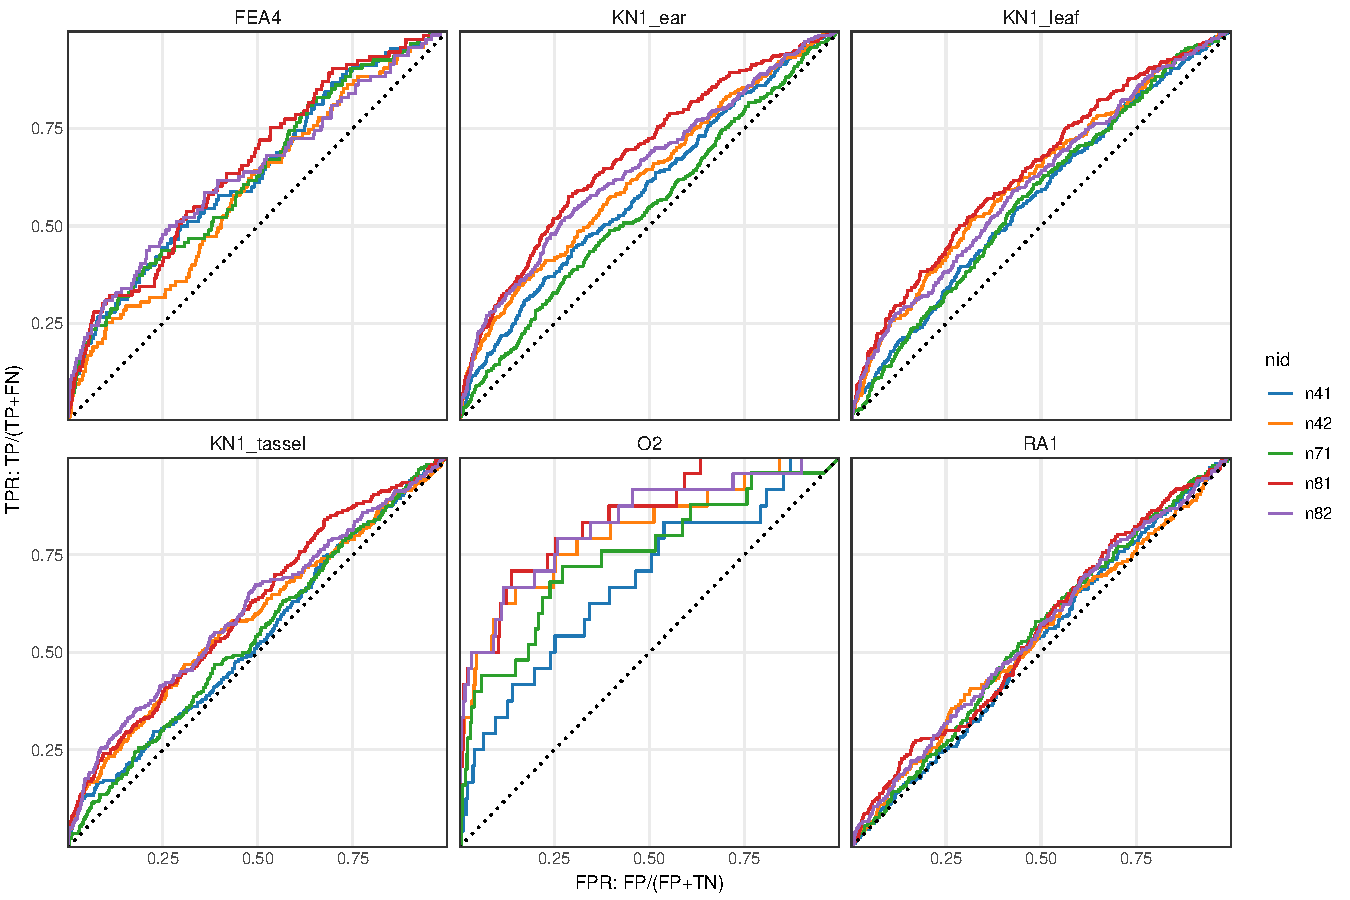
\includegraphics[width=1\textwidth,height=\textheight]{$grn/data/13_auroc/10.dev.atlas.pdf}
\caption{Fig 1}
\end{figure}

Area under receiver operating curves (AUROC) and area under
precision-recall curve (AUPR) for GRNs built using different input
datasets evaluated using experimentally (Chip-seq, mutant \& wildtype
RNA-Seq) determined transcription factor (TF) targets.

\pagebreak

\begin{figure}
\centering
\includegraphics[width=1\textwidth,height=\textheight]{$grn/data/13_auroc/05.auc.lin2017.pdf}
\caption{Fig 2}
\end{figure}

Barplot showing AUROC and AUPRs for lin2017 tissue-specific and pooled
GRNs.

\pagebreak

\begin{figure}
\centering
\includegraphics[width=1\textwidth,height=\textheight]{$grn/data/13_auroc/05.auc.kremling2018.pdf}
\caption{Fig 3}
\end{figure}

Barplot showing AUROC and AUPRs for kremling2018 tissue-specific and
pooled GRNs.

\pagebreak

\begin{figure}
\centering
\includegraphics[width=1\textwidth,height=\textheight]{$grn/data/13_auroc/05.auc.all.pdf}
\caption{Fig 4}
\end{figure}

Barplot showing AUROC and AUPRs for all GRNs.

\pagebreak

\begin{figure}
\centering
\includegraphics[width=1\textwidth,height=\textheight]{$grn/data/13_auroc/06.pcc.lin2017.pdf}
\caption{Fig 5}
\end{figure}

Barplots showing AUROC and AUPRs for PCC-based TF-target prediction
(ranked by PCC).

\pagebreak

\begin{figure}
\centering
\includegraphics[width=1\textwidth,height=\textheight]{$grn/data/13_auroc/06.pcc.kremling2018.pdf}
\caption{Fig 6}
\end{figure}

Barplot showing AUROC and AUPRs for PCC-based TF-target prediction
(ranked by PCC).

\pagebreak

\begin{figure}
\centering
\includegraphics[width=1\textwidth,height=\textheight]{$grn/data/13_auroc/06.pcc.all.pdf}
\caption{Fig 7}
\end{figure}

Barplot showing AUROC and AUPRs for PCC-based TF-target prediction
(ranked by PCC).

\pagebreak

\begin{figure}
\centering
\includegraphics[width=1\textwidth,height=\textheight]{$grn/data/15_de_val/03.lin2017.pdf}
\caption{Fig 8}
\end{figure}

Enrichment of DE genes (using Briggs dataset) in predicted TF targets
made by different GRNs.

\pagebreak

\begin{figure}
\centering
\includegraphics[width=1\textwidth,height=\textheight]{$grn/data/15_de_val/03.kremling2018.pdf}
\caption{Fig 9}
\end{figure}

Enrichment of DE genes (using Briggs dataset) in predicted TF targets
made by different GRNs.

\pagebreak

\begin{figure}
\centering
\includegraphics[width=1\textwidth,height=\textheight]{$grn/data/15_de_val/03.all.pdf}
\caption{Fig 10}
\end{figure}

Enrichment of DE genes (using Briggs dataset) in predicted TF targets
made by different GRNs.
\newpage
\singlespacing 
\end{document}

